\section{Results}\label{sec:results}

This section reports the confirmation map: all \CellsAll{} cells on \NumSeeds{} seeds never run before
the freeze, with \NumPeople{} people, read once and as registered. Numbers come from it unless stated
otherwise. Figure~\ref{fig:grid} shows every cell in the space of the three controls.

The section has three steps. First, what the arrangement does with no distress: the payments that go
unpaid, what households gain, and where the gain comes from. Second, what demurrage does within it: the
price and availability of bridging, the speed of circulation, and the equations of Section~\ref{sec:implications}
set against the simulation. Third, the registered claim and where it ends: the cells where it holds, the
edge at low outside rates, distress, and the record rule for how savers enter the pool.
Section~\ref{sec:robustness} then reports the checks beside the map.

\begin{figure}[htbp]\centering
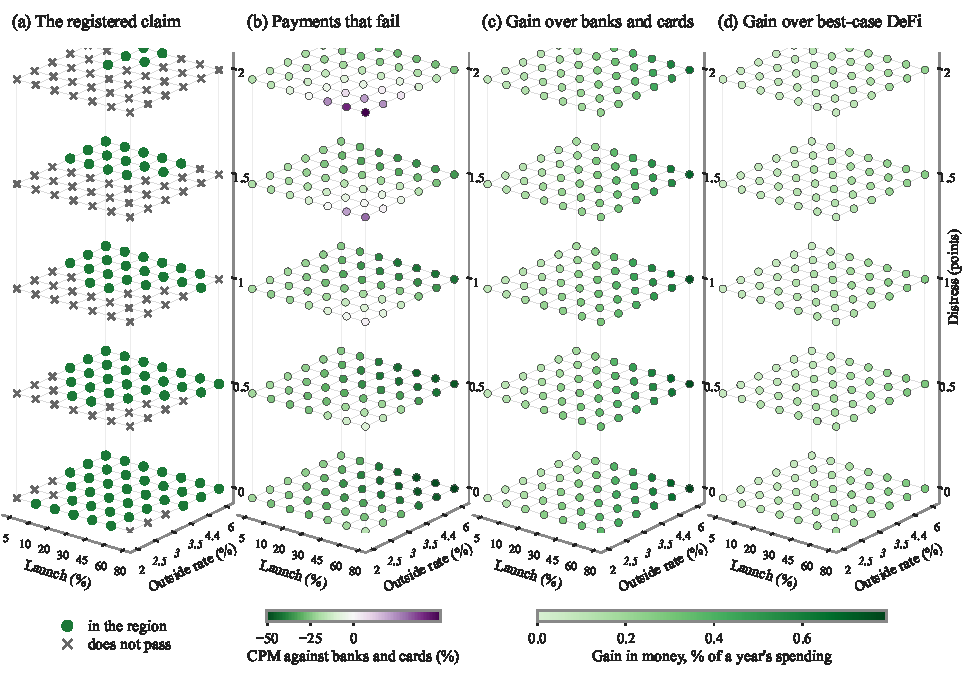
\includegraphics[width=\linewidth]{figures/fig_grid.pdf}
\caption{The whole experiment in the space of its three controls. Each marker is one cell: a launch participation,
an outside rate and a level of distress, read on its seeds; each layer is one level of distress. (a) The registered
claim: the cells in the region of their map. (b) CPM's share of payments that fail against that of banks and
cards, as a relative difference: green where CPM's is lower, purple where higher. (c) and (d) CPM's gain in
money over banks and cards and over best-case DeFi over the sixty months, as a share of a year's spending, on one
scale. The outside rates in italics, 2.5, 3 and 3.5\%, are the exploratory rate cut (Section~\ref{sec:lowrates}) on \CutSeeds{} seeds; the
others are the registered map on \NumSeeds{} seeds.}
\label{fig:grid}
\end{figure}

\subsection{Payments}

Table~\ref{tab:arrangements} and Figure~\ref{fig:failed} give the share of payments that fail: of the value of
bills and purchases due in years 4 and 5, the part not paid on its due day. Wages are counted
apart, below. With no distress the share is \FailBanksMean{} under banks and cards and
\FailDefiMean{} under best-case DeFi, against \FailPoolMean{} with the pool without the charge and \FailCpmMean{}
under CPM, as means over the \CellsNoDistress{} cells. CPM's share is \FailCutBanks{} below that of banks and
cards and \FailCutDefi{} below best-case DeFi's. The pool without the charge is already \FailCutPoolBanks{} below
banks and cards. On this measure the pool and its credit do most of the work; what demurrage adds is the
price of that credit and the cash kept ready for it (Section~\ref{sec:demurrage}). The gap to both
alternatives opens with launch participation, since only a participant can draw a bridge, and is present at
every outside rate. Best-case DeFi stays close to banks and cards at every level: it moves payments and pays a
yield but does nothing for a payer who is short.

Each person pays 58.3\% of its spending as a wage to another. A wage not paid on
its due date stays owed and is paid later, so it is recorded apart. Taking bills, purchases
and wages together, the value not paid on its first due date is \FailedValueBanks{} a person a year under banks
and cards and \FailedValueCpm{} under CPM. Wages paid late are \FailedWageShareBanks{} of it under banks and
cards and \FailedWageShareCpm{} under CPM; purchases lost are the rest. The unpaid value falls mostly on people without a
card: the \NoCardPeople{} who hold none are the payers of \NoCardFailedShareBanks{} of it
under banks and cards and \NoCardFailedShareCpm{} under CPM. Shortfalls in the model come from the timing of receipts and
payments and from job loss. Unexpected expenses are switched off in every run (Section~\ref{sec:model}), so they do
not drive the need for bridging.

\begin{table}[htbp]\centering\small
\resizebox{\linewidth}{!}{% Written by scripts/paper_numbers.py from confirmation_quote.
\begin{tabular}{lrrrrr}
\toprule
Arrangement & Failed, none (mean) & Failed, none (range) & Failed, 2 points (mean) & Failed, 2 points (range) & Purchases completed (\$ a person a year) \\
\midrule
Banks and cards & 3.641\% & 3.585\% to 3.691\% & 5.916\% & 5.757\% to 6.058\% & \$31{,}124 \\
Best-case DeFi & 3.530\% & 3.264\% to 3.630\% & 5.655\% & 5.156\% to 5.887\% & \$31{,}137 \\
Pool without the holding charge & 2.453\% & 1.968\% to 3.069\% & 4.968\% & 4.312\% to 6.654\% & \$31{,}424 \\
CPM & 2.373\% & 1.826\% to 2.997\% & 4.919\% & 4.204\% to 6.773\% & \$31{,}452 \\
Indexed CPM & 2.362\% & 1.816\% to 2.968\% & 4.893\% & 4.195\% to 6.645\% & \$31{,}454 \\
\bottomrule
\end{tabular}
}
\caption{Payments that fail: the value of bills and purchases not paid on their due day, as a share of the value
due in years 4 and 5 (wages counted apart), with no distress and at 2 points of distress, by
arrangement: the mean and the range over cells of the seed means. The last column is purchases completed.}
\label{tab:arrangements}
\end{table}

\begin{figure}[htbp]\centering
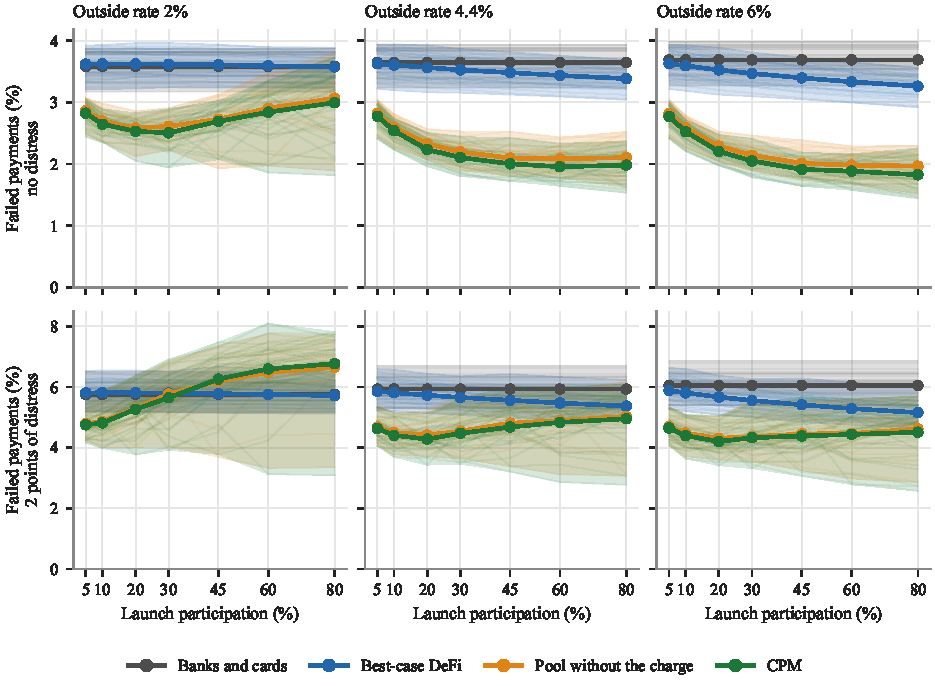
\includegraphics[width=\linewidth]{figures/fig_failed_payments.pdf}
\caption{Payments that fail against launch participation, by outside rate, with no distress (top) and at 2 points
of distress (bottom). Thick lines are seed means, bands the range of the seeds and thin lines the single seeds. Under
distress at high launch the seeds part, and the mean is the path of none of them.}
\label{fig:failed}
\end{figure}

\subsection{Gains}

Figure~\ref{fig:gains} and Table~\ref{tab:gains} give CPM's gain per person per year. A person in the model
stands for one United States consumer unit, so a figure per person is per household. Against banks and
cards the
median over cells is \GainBanksMedian{} in money alone and \GainBanksFaceMedian{} with completed purchases
counted at their price. Against best-case DeFi the two are \GainDefiMedian{} and \GainDefiFaceMedian{}. The
gain is positive in every cell at both ends of the bracket. It stays positive in every cell when the cash-advance
fees and interest CPM saves are taken out: the lowest cell then reads \GainBanksBoundLow{} against banks and
cards and \GainDefiBoundLow{} against best-case DeFi, in money alone. In
\CellsGainPositive{} of the \CellsAll{} cells, at every level of distress, CPM's mean gain over both
alternatives is positive in money alone, with completed purchases counted, and under the cash-advance bound.

The same result can be stated without dollars, which depend on the model's unit, a month of mean spending of
\$6,440. As a share of a year's spending the gain in money is \GainBanksSpending{} over banks and cards and
\GainDefiSpending{} over best-case DeFi, and \GainBanksFaceSpending{} and \GainDefiFaceSpending{} with completed
purchases at their price. A larger number is the change in what households pay intermediaries outside the
household economy, net of what those pay back: interest and the cash-advance and late fees of outside lenders,
failure fees, card fees less rewards, the spread banks and funds keep on balances and, under CPM, the issuer's custody, the pool's
operating cost and gas. At the median cell it is \OutsidePaidBanks{} a person a year under banks and cards,
\OutsidePaidDefi{} under best-case DeFi and \OutsidePaidCpm{} under CPM. Cell by cell CPM cuts it by a median of
\OutsideCutBanks{} against banks and cards, from \OutsideCutBanksLow{} at the lowest launch level to
\OutsideCutBanksHigh{} at the highest, and by \OutsideCutDefi{} against best-case DeFi. Without the spread on
balances, which is yield forgone and not cash paid, the cut against banks and cards is \OutsideCashCutBanks{}.
These payments are transfers, not resources used; the efficiency reading is the real cost below.

These are averages over people, and the average is above the typical person. In money alone the median person at
the median cell gains \PersonMedianBanks{} a year over banks and cards and \PersonMedianDefi{} over best-case
DeFi, \PersonMedianBanksSpending{} and \PersonMedianDefiSpending{} of a year's spending and less than half the
mean. At the fifth percentile the gain is \PersonFifthBanks{} and
\PersonFifthDefi{} a year. In money alone
\ShareBehindBanksMoney{} of people end more than \$2 a year behind the bank arrangement and
\ShareBehindDefiMoney{} behind best-case DeFi; with completed purchases at their price the shares are
\ShareBehindBanks{} and \ShareBehindDefi{} (Table~\ref{tab:gains}). The claim's group clause reads the mean of
each group, not each person.

In real resources CPM uses less than banks and cards in every cell, by at least \RealCostBanksLow{} a person a
year. Against best-case DeFi the difference is small in every cell, from \RealCostDefiLow{} to
\RealCostDefiHigh{} a person a year, with CPM using slightly more at the highest launch levels
(Table~\ref{tab:gains}). So the gain over best-case DeFi is the credit the pool supplies, apart from
0.20 point of yield on balances, which the custody check of Section~\ref{sec:robustness} removes without changing
the sign. It is not a cheaper way of moving money.

Two read-outs stored with the real cost say the same in other units. The model costs each payment the pool
rescues at \$2, as it does a failed one. CPM would use the same real resources as best-case DeFi if a rescue cost
between \RescueEvenDefiLow{} and \RescueEvenDefiHigh{} across the cells with no distress (median
\RescueEvenDefiMedian{}), and the same as banks and cards if it cost between \RescueEvenBanksLow{} and
\RescueEvenBanksHigh{} (median \RescueEvenBanksMedian{}). Against banks and cards the comparison has room to
spare; against best-case DeFi it rests on what a rescue is taken to cost. For each dollar of purchases completed
the real cost is \CentsCompletedBanks{} cents under banks and cards, \CentsCompletedDefi{} under best-case DeFi
and \CentsCompletedCpm{} under CPM, on average over the same cells.

\begin{figure}[htbp]\centering
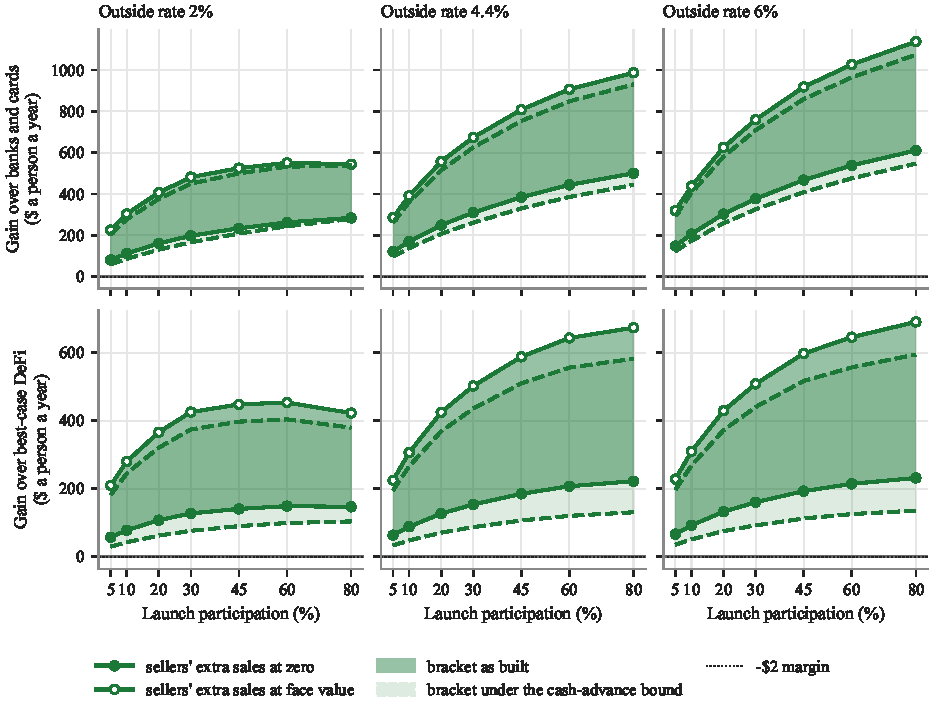
\includegraphics[width=\linewidth]{figures/fig_gains.pdf}
\caption{CPM's gain per person per year against banks and cards (top) and against best-case DeFi (bottom), by
outside rate, with no distress. The band runs from the gain in money alone to the gain with completed purchases at
their price; the dashed band is the same under the cash-advance bound.}
\label{fig:gains}
\end{figure}

\begin{table}[htbp]\centering\small
\resizebox{\linewidth}{!}{% Written by scripts/paper_numbers.py from confirmation_quote.
\begin{tabular}{lrrrr}
\toprule
 & Banks (median) & Banks (range) & DeFi (median) & DeFi (range) \\
\midrule
Wealth gain & \$262 & \$80 to \$610 & \$140 & \$57 to \$231 \\
Complete gain at face value & \$550 & \$225 to \$1{,}138 & \$429 & \$209 to \$690 \\
Complete gain at zero & \$262 & \$80 to \$610 & \$140 & \$57 to \$231 \\
Wealth gain under the cash-advance bound & \$243 & \$59 to \$547 & \$87 & \$29 to \$135 \\
Complete gain at face, under the bound & \$532 & \$204 to \$1{,}074 & \$379 & \$182 to \$594 \\
Complete gain at zero, under the bound & \$243 & \$59 to \$547 & \$87 & \$29 to \$135 \\
Cash-advance fees and interest saved & \$33 & \$5.3 to \$64 & \$51 & \$27 to \$96 \\
Real cost saved & \$18 & \$4.7 to \$40 & $-$\$0.1 & $-$\$2.0 to \$0.2 \\
Share below $-$\$2 a year, complete gain at face & 10.6\% & 9.2\% to 17.7\% & 13.2\% & 11.5\% to 20.3\% \\
Wealth gain read at month 36 & \$221 & \$45 to \$560 & \$114 & \$30 to \$208 \\
Wealth gain read at month 48 & \$263 & \$61 to \$589 & \$135 & \$42 to \$221 \\
\midrule
Lowest group lower bound, as built & \multicolumn{4}{l}{\$0.5} \\
Lowest group lower bound, under the bound & \multicolumn{4}{l}{$-$\$2.6} \\
\midrule
Clause (a) & \multicolumn{4}{l}{21 of 21} \\
Clause (b) & \multicolumn{4}{l}{20 of 21} \\
Clause (c), reported & \multicolumn{4}{l}{21 of 21} \\
Clause (d) as built & \multicolumn{4}{l}{21 of 21} \\
Clause (d) under the bound & \multicolumn{4}{l}{20 of 21} \\
All of (a), (b), (d) as built & \multicolumn{4}{l}{20 of 21} \\
All of (a), (b), (d) under the bound & \multicolumn{4}{l}{19 of 21} \\
All, as built and under the bound & \multicolumn{4}{l}{19 of 21} \\
In the region (largest joined block) & \multicolumn{4}{l}{19 of 21} \\
\bottomrule
\end{tabular}
}
\caption{CPM against banks and cards and against best-case DeFi over the \CellsNoDistress{} cells with no distress,
in dollars a person a year: median and range over cells. The lower block counts the cells where each clause of
the registered claim passes on the \NumSeeds{} confirmation seeds.}
\label{tab:gains}
\end{table}

\subsection{Where the gain comes from}

Table~\ref{tab:sources} splits CPM's gain in money over banks and cards by the flow it comes from, at each outside
rate with no distress. The split is an accounting identity: in every cell its lines add up to the gain. Four lines
carry it. The reserve return paid on P is \SourceYieldTwo{} a person a year at an outside rate of 2\%,
\SourceYieldFourFour{} at 4.4\% and \SourceYieldSix{} at 6\%, or \SourceYieldShareTwo{},
\SourceYieldShareFourFour{} and \SourceYieldShareSix{} of the gain. Interest no longer paid to cards and outside
lenders, because the pool lent instead and its interest stays with the households that own it, is
\SourceInterestTwo{}, \SourceInterestFourFour{} and \SourceInterestSix{}, or \SourceInterestShareTwo{},
\SourceInterestShareFourFour{} and \SourceInterestShareSix{} of the gain. Cash-advance, late and failure fees saved are \SourceFeesTwo{},
\SourceFeesFourFour{} and \SourceFeesSix{}, and card fees saved, less the rewards given up, about
\SourceCardFourFour{} at every rate. Against them stand the pool's operating cost and the savings income given up
on money moved into P and the pool.

The reserve return moves most with the outside rate; the fees saved also nearly double between 2\% and 4.4\%. Best-case DeFi also pays its holders a return on the
reserve and moves money off the card rails, so of these lines the two that come from credit, the interest and the
fees saved, separate CPM from it. That is why the gain over best-case DeFi is the smaller of the two and
changes less with the outside rate (Figure~\ref{fig:gains}). The reserve return is also one of the two reasons the
claim is weakest at low outside rates (Section~\ref{sec:lowrates}).

\begin{table}[htbp]\centering\small
% Written by scripts/paper_numbers.py from confirmation_quote.
\begin{tabular}{lrrr}
\toprule
Outside rate & 2.0\% & 4.4\% & 6.0\% \\
\midrule
Reserve return on P and other outside income & \$55 & \$138 & \$194 \\
Interest saved on outside loans & \$102 & \$118 & \$133 \\
Card fees saved, less rewards given up & \$41 & \$42 & \$42 \\
Cash-advance, late and failure fees saved & \$34 & \$65 & \$69 \\
The pool's operating cost & $-$\$22 & $-$\$17 & $-$\$17 \\
Savings income given up, inflation and valuation & $-$\$22 & $-$\$35 & $-$\$43 \\
Conversion fees, gas and wages to the outside & $-$\$1.8 & $-$\$1.6 & $-$\$1.6 \\
\midrule
Gain over banks and cards & \$197 & \$309 & \$376 \\
\bottomrule
\end{tabular}

\caption{CPM's gain in money over banks and cards by the flow it comes from, in dollars a person a year: the median
over the seven launch levels at each outside rate, with no distress. The lines add up to the gain in each cell;
medians over cells need not add up exactly.}
\label{tab:sources}
\end{table}

Figure~\ref{fig:sources} gives the same split in every cell, in dollars and as shares of the cell's gain. As launch
participation rises, card fees saved take a larger share of the gain and the fees saved on shortfalls a smaller
one; the shares of the reserve return and of the interest move less.

\begin{figure}[htbp]\centering
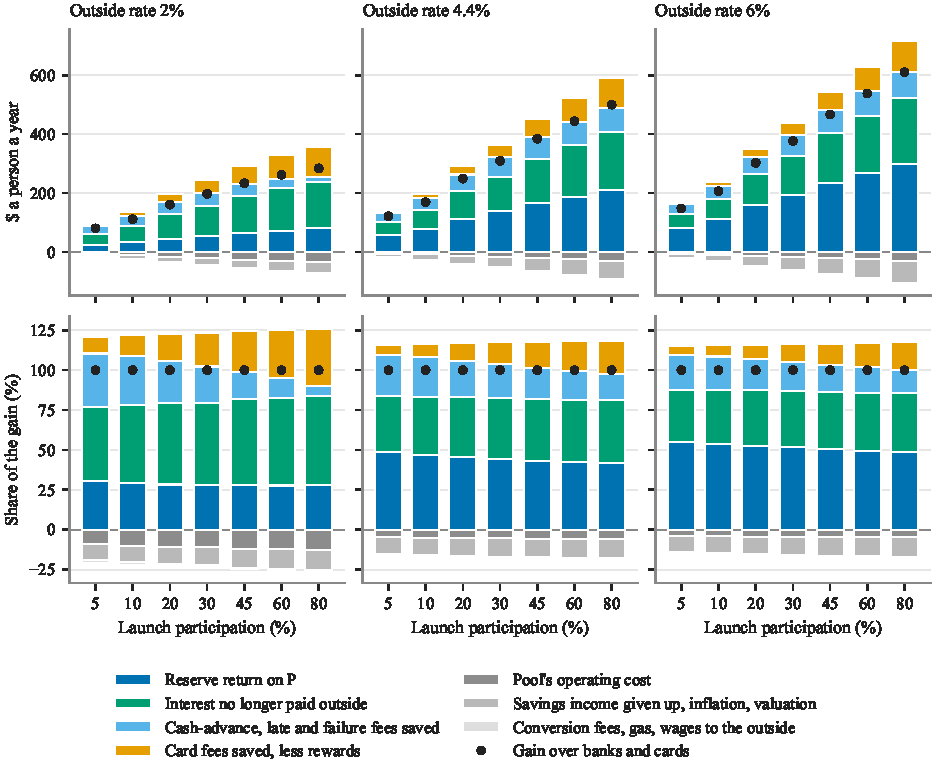
\includegraphics[width=\linewidth]{figures/fig_sources.pdf}
\caption{CPM's gain in money over banks and cards by the flow it comes from, in each of the \CellsNoDistress{} cells
with no distress: dollars a person a year (top) and each flow as a share of the cell's gain (bottom). Costs are
stacked below zero and the dot marks the gain.}
\label{fig:sources}
\end{figure}

\subsection{What demurrage does}\label{sec:demurrage}

The pool without the charge is the same money and the same pool on the same people and draws, so its difference
from CPM is what demurrage does (Tables~\ref{tab:buys} and~\ref{tab:charge}, Figure~\ref{fig:charge}).

The demurrage rate is \ChargeFrom{} to \ChargeTo{} a year across cells. At the median cell the holding charge costs holders
\ChargeDollars{} a person a year, and Table~\ref{tab:buys} sets beside that cost what it pays for. The price a
bridge borrower pays falls from between \BridgePricePoolLow{} and \BridgePricePoolHigh{}, depending on the outside
rate, to \BridgePriceCpm{} at every rate, a cut of \BridgeCutLow{} to \BridgeCutHigh{}, as
equation~\eqref{eq:bridgeprice} requires: the capital part of the coupon moves from the borrower to all holders.
The pool keeps \StandbyChange{} more cash standing by, \StandbyCpm{} a person against \StandbyPool{}, because its
capital target now includes cash against the peak of bridging, and serves a larger share of the bridges asked
of it at every outside rate. Bridging by the pool rises by \PoolBridgingChange{}, from \PoolBridgingPool{} to
\PoolBridgingCpm{} a person a year. Balances revolved on cards fall by \RevolvedChange{}, from \RevolvedPool{} to
\RevolvedCpm{}, and the value of payments that fail from \FailedDollarsPool{} to \FailedDollarsCpm{}.

By Corollary~\ref{cor:neutral} the charge cannot create wealth at fixed quantities: what holders pay, borrowers
and owners receive. So CPM's net gain over the pool without the charge is the value of the quantities
that changed. At the median cell it is \GainOverPool{} a person a year over the whole run and
\GainOverPoolLate{} in years 4 and 5, when the charge collected is \ChargeDollars{}: household
wealth is \GainPerChargeDollar{} dollars higher for each dollar collected. That compares two runs; it is not
a payment the contract makes. The size check (Section~\ref{sec:robustness}) shows the gain still grows
with the population. Demurrage here is insurance
and is priced like it: a small premium on every balance, paid out as cheap and available credit to whoever
is short.

In dollars this is the smallest gain the paper reports, so it is read with its interval. CPM and the pool without
the charge run on the same people and draws, and their difference is paired seed by seed.
Table~\ref{tab:chargegain} and Figure~\ref{fig:chargegain} give it at every distress level (Section~\ref{sec:stress}). Under the quote rule, where savers enter on the
pool's published quote, the median over cells is
\ChargeGainFirstMedianZero{} a person a year with no distress and \ChargeGainFirstMedianTwo{} at 2 points. The
lower end of the 95\% interval across seeds is above zero in \ChargeGainFirstAboveAll{} of the
\ChargeGainFirstCells{} cells of the grid; the lowest, at 2 points, is \ChargeGainFirstLowTwo{}. CPM fails fewer
payments than the pool without the charge in \ChargeGainFirstFewerAll{} of those cells. Under the record rule,
where they enter on its realised return (Section~\ref{sec:record}), the medians are \ChargeGainSecondMedianZero{} and
\ChargeGainSecondMedianTwo{}, the lower end is above zero in \ChargeGainSecondAboveAll{} cells and CPM fails fewer
payments in \ChargeGainSecondFewerAll{}. These intervals are not part of the registered claim and carry no
correction for the number of cells.

\begin{table}[htbp]\centering\small
\resizebox{\linewidth}{!}{% Written by scripts/paper_numbers.py from confirmation_quote.
\begin{tabular}{lrrrrrrrr}
\toprule
 & \multicolumn{4}{c}{Quote rule} & \multicolumn{4}{c}{Record rule} \\
Distress & Median gain & Lowest lower bound & Cells above zero & Cells with fewer failures & Median gain & Lowest lower bound & Cells above zero & Cells with fewer failures \\
\midrule
0 pt & \$15 & \$4.9 & 21 & 21 & \$61 & \$34 & 21 & 21 \\
0.5 pt & \$15 & \$4.7 & 21 & 21 & \$56 & \$35 & 21 & 21 \\
1 pt & \$13 & \$4.6 & 21 & 19 & \$53 & \$32 & 21 & 19 \\
1.5 pt & \$13 & \$3.8 & 21 & 18 & \$50 & \$27 & 21 & 18 \\
2 pt & \$12 & \$0.1 & 21 & 18 & \$46 & \$21 & 21 & 15 \\
\bottomrule
\end{tabular}
}
\caption{CPM's gain in money over the pool without the charge, in dollars a person a year, by distress level and
under the two entry rules: the median over the \CellsNoDistress{} cells of each level; the lowest,
over those cells, of the lower end of the 95\% interval of the paired gain across the \NumSeeds{} seeds; the cells
where that lower end is above zero; and the cells where CPM fails fewer payments than the pool without the
charge.}
\label{tab:chargegain}
\end{table}

\begin{figure}[htbp]\centering
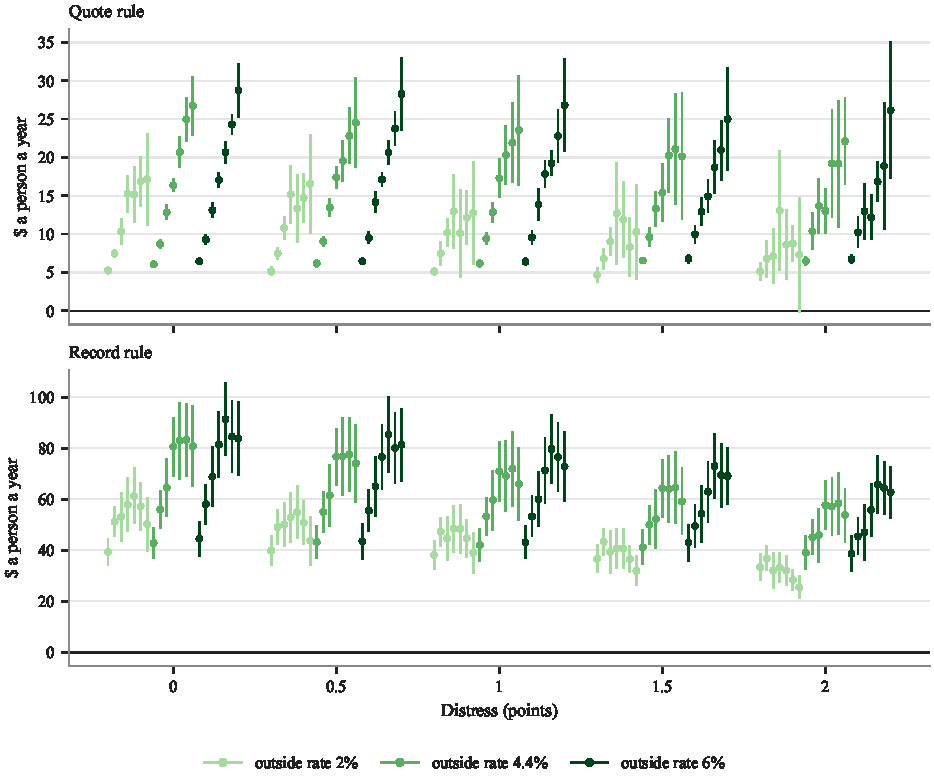
\includegraphics[width=\linewidth]{figures/fig_charge_gain.pdf}
\caption{CPM's gain in money over the pool without the charge in every cell of the grid: the mean across the
\NumSeeds{} seeds and its 95\% interval, by distress level, under the quote rule (top) and the record rule
(bottom). Within a level the cells run by outside rate and then by launch participation.}
\label{fig:chargegain}
\end{figure}

Table~\ref{tab:buys} also measures liquidity support across arrangements. Banks and cards hold \PrecautionBanks{} dollars of
precautionary money for each dollar of shortfall a lender covers in a year, and best-case DeFi \PrecautionDefi{}.
The pool holds \PrecautionPool{} without the charge and \PrecautionCpm{} with it, and covers more shortfalls than
either. Each dollar of precautionary money covers more shortfall once part of it is pooled; households' own
buffers are no smaller (Table~\ref{tab:buys}).

\begin{table}[htbp]\centering\small
\resizebox{\linewidth}{!}{% Written by scripts/paper_numbers.py from confirmation_quote.
\begin{tabular}{lrrrr}
\toprule
 & Banks and cards & Best-case DeFi & Pool without the holding charge & CPM \\
\midrule
Demurrage paid by holders, \$ a person a year &  &  & \$0.0 & \$4.7 \\
Bridge price to the borrower, \% a year &  &  & 6.7\% & 2.1\% \\
Shortfalls a lender covered, \$ a person a year & \$2{,}783 & \$3{,}119 & \$4{,}879 & \$5{,}015 \\
\quad by the pool & \$0.0 & \$0.0 & \$2{,}645 & \$2{,}982 \\
\quad on the card & \$1{,}868 & \$2{,}198 & \$1{,}407 & \$1{,}357 \\
\quad revolved on the card & \$872 & \$907 & \$706 & \$637 \\
Payments that failed, \$ a person a year & \$3{,}042 & \$3{,}006 & \$2{,}147 & \$2{,}094 \\
Precautionary money held, \$ a person & \$1{,}289 & \$1{,}726 & \$1{,}740 & \$1{,}742 \\
\quad of which pool cash standing by & \$0.0 & \$0.0 & \$31 & \$50 \\
Precautionary money per dollar of shortfall covered & 0.46 & 0.54 & 0.36 & 0.36 \\
Gain over the pool without the charge, \$ a person a year &  &  &  & \$15 \\
\bottomrule
\end{tabular}
}
\caption{What demurrage buys, and liquidity support by arrangement: medians over the cells with no
distress, years 4 and 5. A shortfall is what a payer's own money and same-day savings could not pay; a lender
covers it through the pool, the card, a balance revolved on the card or earned-wage access. Precautionary money
is households' chosen buffers and the pool's idle cash.}
\label{tab:buys}
\end{table}

\begin{table}[htbp]\centering\small
\resizebox{\linewidth}{!}{% Written by scripts/paper_numbers.py from confirmation_quote.
\begin{tabular}{llrrrrrrr}
\toprule
Outside rate & Arrangement & Bridge price & Gross coupon & Bridges served & Demurrage $c$ & $\theta$ & Payments that fail & Gain over the pool without the charge \\
\midrule
2.0\% & Pool without the holding charge & 4.34\% & 4.34\% & 0.675 & 0.000\% & 0.000 & 2.728\% &  \\
2.0\% & CPM & 2.10\% & 4.34\% & 0.758 & 0.070\% & 0.518 & 2.693\% & \$15 \\
4.4\% & Pool without the holding charge & 6.75\% & 6.75\% & 0.792 & 0.000\% & 0.000 & 2.198\% &  \\
4.4\% & CPM & 2.09\% & 6.74\% & 0.872 & 0.137\% & 0.690 & 2.106\% & \$16 \\
6.0\% & Pool without the holding charge & 8.34\% & 8.34\% & 0.800 & 0.000\% & 0.000 & 2.144\% &  \\
6.0\% & CPM & 2.08\% & 8.33\% & 0.880 & 0.177\% & 0.750 & 2.051\% & \$17 \\
\bottomrule
\end{tabular}
}
\caption{CPM against the pool without the charge, with no distress, by outside rate: medians over launch levels of
the seed means in years 4 and 5.}
\label{tab:charge}
\end{table}

\begin{figure}[htbp]\centering
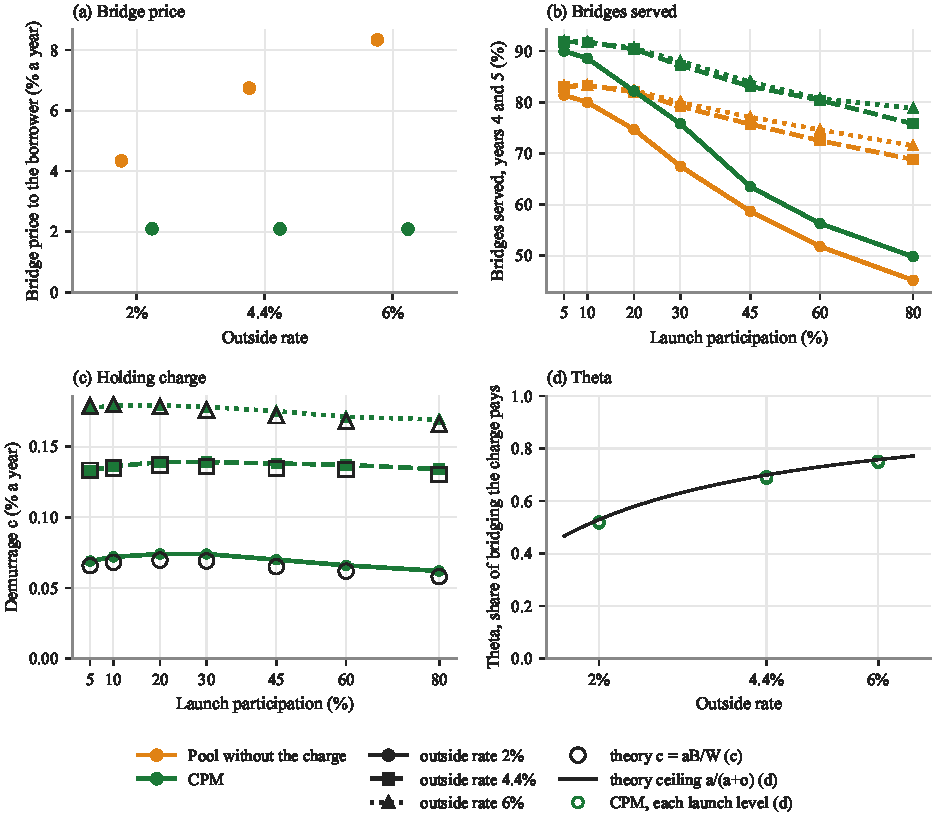
\includegraphics[width=\linewidth]{figures/fig_charge.pdf}
\caption{What demurrage does. (a) The price a bridge borrower pays. (b) Bridges served. (c) The charge,
with the value $a\,B/W$ of Proposition~\ref{prop:size} where the stored fields allow. (d) The charge's share of
bridging finance against its ceiling $a/(a+o)$.}
\label{fig:charge}
\end{figure}

\subsection{Circulation}

The arrangement's name invites a question its mechanism does not depend on: whether a charge on balances makes
money move faster. We measure circulation with MicroVelocity \cite{campajola} in years 4 and 5
(Table~\ref{tab:circulation}, Figure~\ref{fig:circulation}). A unit of money held for $\tau$ days between
receipt and spending adds $1/\tau$ for each day it is held; a person's MicroVelocity is that sum over the
money it holds, divided by the total stock of money, so people's MicroVelocities add up to the velocity of
money. Money spent is matched to money received last in first out, as in \cite{decollibus}, with first in first
out beside it, and money not spent again within the run is left out, as in both papers. Wallet turnover is
also reported: a person's payments to others over a year divided by its own average balance of bank money
and $P$, the inverse of its average holding time. The time between
receipt and spending is the holding time of \cite{campajola}; \cite{zhang} call it the lifespan.

Gesell's demurrage \cite{gesell} was meant to make money circulate faster. This one does not speed circulation by
any amount that matters. Under CPM the money a participant spends has been
held for \HoldingDaysCpm{} days on average, against \HoldingDaysPool{} days in the pool without the charge, and the
velocity of all money is \VelocityCpm{} turns a year against \VelocityPool{}. The differences have a consistent
sign and are about one per cent. The size of the charge implies as much: a fraction of a percentage
point a year gives nobody a reason to spend sooner. The demurrage works through the price and availability of
bridging, as Section~\ref{sec:implications} derives, not through the speed of spending.

The pool, with or without the charge, does change the measure. The velocity of all money is \VelocityBanks{} turns
a year under banks and cards and \VelocityDefi{} under best-case DeFi, against \VelocityCpm{} under CPM. The measure counts bank money, $P$ and
outside savings. Spare money placed in the pool is lent on and spent, where spare money in outside savings
sits, so a smaller stock of money carries the same spending. The rise reflects where spare money rests,
not people spending faster. Circulation is no more concentrated under the pool: the tenth of
people who contribute most to velocity carry about a quarter of it in every arrangement.

\begin{table}[htbp]\centering\footnotesize
\resizebox{\linewidth}{!}{% Written by scripts/paper_numbers.py from confirmation_quote.
\begin{tabular}{lllllrr}
\toprule
 & Statistic & Unit & Arrangement & People & Median & Range \\
\midrule
(a) & Wallet turnover, median person & turns a year & Banks and cards & everyone & 49.6 & 48.5 to 49.9 \\
 &  &  & Best-case DeFi & participants & 19.8 & 18.7 to 20.0 \\
 &  &  & Pool without the holding charge & participants & 24.0 & 22.5 to 27.8 \\
 &  &  & CPM & participants & 24.0 & 22.6 to 28.1 \\
\midrule
(a) & Wallet turnover, balance-weighted mean & turns a year & Banks and cards & everyone & 47.6 & 46.6 to 47.9 \\
 &  &  & Best-case DeFi & participants & 13.4 & 12.7 to 13.7 \\
 &  &  & Pool without the holding charge & participants & 15.7 & 15.2 to 18.3 \\
 &  &  & CPM & participants & 15.8 & 15.3 to 18.5 \\
\midrule
(b) & MicroVelocity, top tenth's share of the group's sum & share & Banks and cards & everyone & 0.255 & 0.254 to 0.255 \\
 &  &  & Best-case DeFi & participants & 0.242 & 0.237 to 0.246 \\
 &  &  & Pool without the holding charge & participants & 0.244 & 0.243 to 0.245 \\
 &  &  & CPM & participants & 0.243 & 0.243 to 0.246 \\
\midrule
(b) & MicroVelocity, median person & turns a year & Banks and cards & everyone & 0.00201 & 0.00199 to 0.00203 \\
 &  &  & Best-case DeFi & participants & 0.00238 & 0.00225 to 0.00269 \\
 &  &  & Pool without the holding charge & participants & 0.00251 & 0.00226 to 0.00314 \\
 &  &  & CPM & participants & 0.00253 & 0.00227 to 0.00315 \\
\midrule
(b) & Aggregate velocity, MicroVelocity summed over everyone & turns a year & Banks and cards & everyone & 10.32 & 10.18 to 10.41 \\
 &  &  & Best-case DeFi & everyone & 10.64 & 10.46 to 11.44 \\
 &  &  & Pool without the holding charge & everyone & 12.48 & 11.07 to 15.57 \\
 &  &  & CPM & everyone & 12.54 & 11.13 to 15.76 \\
\midrule
(c) & Mean holding time of money spent, last in first out & days & Banks and cards & everyone & 26.5 & 26.2 to 26.7 \\
 &  &  & Best-case DeFi & participants & 29.5 & 27.2 to 31.9 \\
 &  &  & Pool without the holding charge & participants & 27.2 & 22.9 to 29.8 \\
 &  &  & CPM & participants & 26.9 & 22.5 to 29.6 \\
\midrule
(c) & Mean holding time of money spent, first in first out & days & Banks and cards & everyone & 34.9 & 34.6 to 35.3 \\
 &  &  & Best-case DeFi & participants & 33.8 & 33.6 to 35.2 \\
 &  &  & Pool without the holding charge & participants & 27.4 & 22.7 to 29.8 \\
 &  &  & CPM & participants & 27.2 & 22.4 to 29.6 \\
\bottomrule
\end{tabular}
}
\caption{Circulation in years 4 and 5 with no distress, by arrangement: median and range over cells of the seed
means. Wallet turnover is a person's outflow over its own average balance of bank money and $P$. MicroVelocity and
holding times are computed from the age of every unit of bank money, $P$ and outside savings when it is spent.
Banks and cards have no network, so their rows cover everyone; the other rows cover each arrangement's
participants unless marked.}
\label{tab:circulation}
\end{table}

\begin{figure}[htbp]\centering
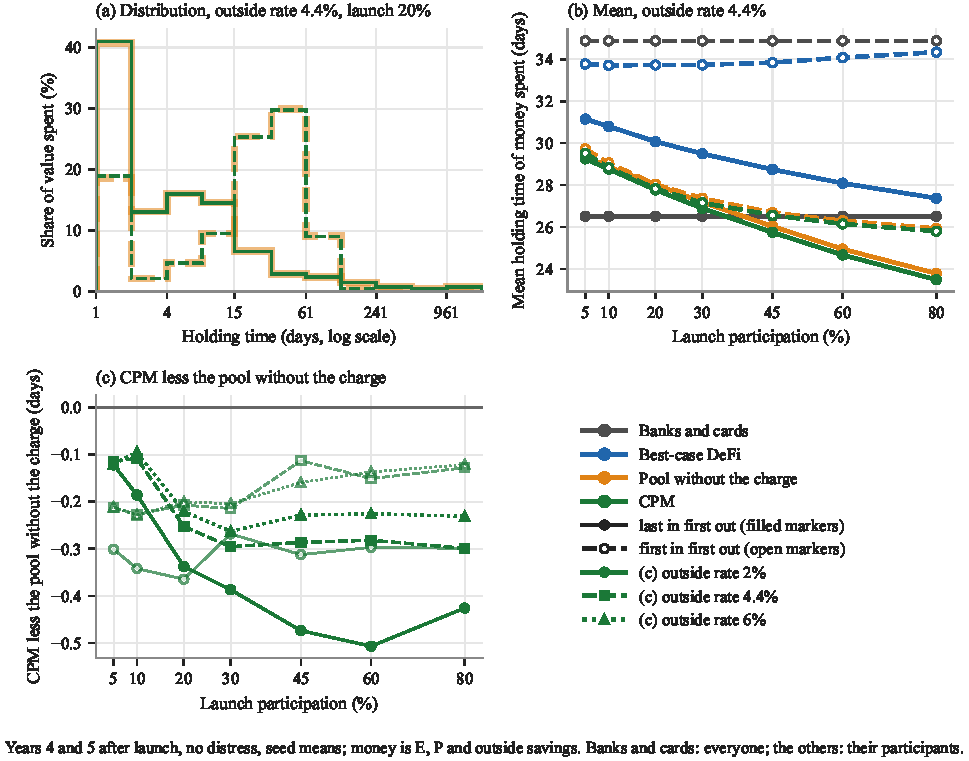
\includegraphics[width=\linewidth]{figures/fig_circulation.pdf}
\caption{Holding times of money spent, years 4 and 5, no distress. (a) The distribution of value spent by holding
time under CPM and under the pool without the charge at one cell. (b) The mean holding time against launch
participation at an outside rate of 4.4\%. (c) CPM less the pool without the charge. Filled markers count the
newest money as spent first, open markers the oldest.}
\label{fig:circulation}
\end{figure}

\subsection{Theory against simulation}

Table~\ref{tab:docking} sets the equations of Section~\ref{sec:implications} beside the simulation over the cells
with no distress, with the largest gap in any cell; its last column says how each row holds. Four rows hold by
construction. The simulation computes the charge, the bridge price and the quote by the contract's own equations,
and the charge's share of bridging finance is a ratio of recorded flows the coupon fixes. These rows check
that the code runs the contract as written and that its records add up. Their value is the size of the
numbers: the charge of Proposition~\ref{prop:size}, computed from the bridge book and wallet balances without its
small standby term, matches the simulated charge, and the share follows Proposition~\ref{prop:theta}. The other
rows predict behaviour. Participation follows the one curve of Proposition~\ref{prop:diffusion}
from every launch level with one fitted leaving rate (Figure~\ref{fig:participation}).

One prediction holds only in part. Proposition~\ref{prop:capital} puts capital at its target when the money offered
exceeds the room. With savers reviewing entry at the monthly rate, offers do not always fill the room, and in the
worst cell capital is below 95\% of its target in the share of seed-months given in the fourth row of
Table~\ref{tab:docking}. The proposition's condition is real, not a formality. Its other half, that
entrants act on the quote, is taken up in Section~\ref{sec:record}.

Proposition~\ref{prop:fair} says the quote is right on average and that an owner's shortfall is a loss tail. Both show.
Owners earn their alternative at the median, with a tail below it. Table~\ref{tab:owners} gives the realised
return on pool capital less the alternative in years 4 and 5 over the seed-cells with no distress. At every
outside rate the median is within \OwnersMedianWorst{} of a percentage point of zero. In one seed-cell in ten
owners fall short of their alternative by \OwnersTenthLeast{} to \OwnersTenthWorst{} of a point a year or more,
depending on the outside rate. The tail matters, because an owner decides whether to stay on its realised
return (Section~\ref{sec:entry}).

\begin{table}[htbp]\centering\small
\resizebox{\linewidth}{!}{% Written by scripts/paper_numbers.py from confirmation_quote.
\begin{tabular}{lrrrl}
\toprule
Quantity & Formula & Simulated & Largest gap & Holds \\
\midrule
Demurrage rate $c = aB/W$ (the standby part $(a - p)S/W$ is not stored), \% a year & 0.058\% to 0.180\% & 0.062\% to 0.179\% & 0.005\% & by construction \\
$\theta = a / r_g$ & 0.517 to 0.751 & 0.517 to 0.751 & 0.002 & by construction \\
Bridge price $= r_g - \kappa a$, \% a year & 2.07\% to 2.12\% & 2.07\% to 2.12\% & 0.00\% & by construction \\
Seed-months with capital below 0.95 of its target & 0.000 & 0.001 to 0.538 & 0.538 & in part \\
Quote at the target $= a$, \% a year & 2.25\% to 6.25\% & 2.24\% to 6.25\% & 0.01\% & by construction \\
Participation at month 12 & 0.098 to 0.853 & 0.099 to 0.849 & 0.014 & as predicted \\
Participation at month 36 & 0.251 to 0.927 & 0.252 to 0.928 & 0.010 & as predicted \\
Participation at month 60 & 0.458 to 0.963 & 0.457 to 0.966 & 0.023 & as predicted \\
\bottomrule
\end{tabular}
}
\caption{Theory against simulation over CPM's cells with no distress: each quantity's formula value and the
simulated value, as ranges over cells, and the largest gap in any cell. A row holds by construction where the
simulation computes the quantity by that equation, as predicted where the equation describes behaviour, and in
part where the prediction's condition is not always met.}
\label{tab:docking}
\end{table}

\begin{figure}[htbp]\centering
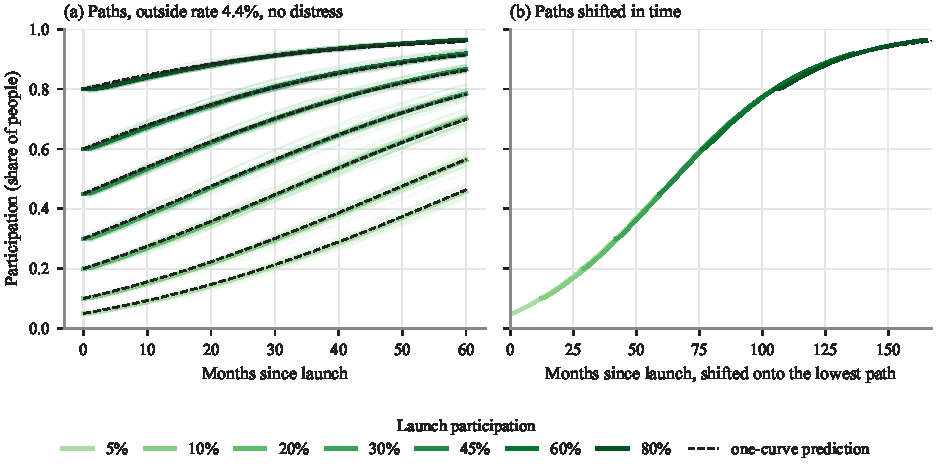
\includegraphics[width=\linewidth]{figures/fig_participation.pdf}
\caption{Participation under CPM at an outside rate of 4.4\% with no distress. (a) Paths from the seven launch
levels, the seed mean thick and each seed thin, with the prediction of equation~\eqref{eq:diffusion}. (b) The
seed-mean paths shifted in time onto the path from the lowest launch level.}
\label{fig:participation}
\end{figure}

\begin{table}[htbp]\centering\small
% Written by scripts/paper_numbers.py from confirmation_quote.
\begin{tabular}{lrrrr}
\toprule
Outside rate & Median & Mean & 10th percentile & Seed-cells with capital \\
\midrule
2.0\% & $-$0.01\% & 0.00\% & $-$0.31\% & 210 of 210 \\
4.4\% & $-$0.01\% & $-$0.09\% & $-$0.52\% & 210 of 210 \\
6.0\% & $-$0.02\% & $-$0.09\% & $-$0.51\% & 210 of 210 \\
\bottomrule
\end{tabular}

\caption{Owners' realised return less their alternative in years 4 and 5, in percentage points a year, over the
seed-cells with no distress.}
\label{tab:owners}
\end{table}

\subsection{The registered claim}

Table~\ref{tab:region} and Figure~\ref{fig:region} give the claim as registered, read once on the \NumSeeds{}
confirmation seeds. With no distress \ClaimCellsAsBuilt{} of the \CellsNoDistress{} cells pass clauses (a), (b) and
(d) as built, and \ClaimCellsBoth{} pass also under the cash-advance bound. Those cells join edge to edge, so the
region is one block of \RegionCellsZero{} cells: every cell at outside rates of 4.4\% and 6\%, and five of the
seven at 2\%. At the Bonferroni level over the \CellsNoDistress{} cells the claim holds in \ClaimHoldsSomewhere{}.
A falsifier fires in \ClaimCellsFalsified{} cell. The seed-count rule marks \ClaimCellsUnderpowered{} cell
underpowered: on the confirmation map's own spreads no cell needs more than \ClaimSeedsCellMost{} seeds, so the
declared extension to \SeedsExtended{} seeds is not used.

In every seed of every cell of the grid the pool forms, households hold at least 90\% of its capital through the
second window and the issuer stays. With no distress at least \SeedsPersistentLeast{} of the \NumSeeds{} seeds are Persistent in every
cell, and clause (a) passes in all of them (Table~\ref{tab:gains}).

The group clause decides little. Against best-case DeFi, with completed purchases at their price, the lowest lower
bound of any group in any cell is \GroupLowDefiFace{} a person a year as built and \GroupLowDefiFaceBound{} under
the bound: every group is ahead of best-case DeFi on the registered clause, by a wide margin. Against banks and
cards the clause is also read at the other end of the bracket, the group's gain in wealth plus the purchases it
received less its own extra sales, so with a seller's extra sales valued at nothing. For a group that is not its
gain in money alone. There the lowest is \GroupLowBanksZero{} as built and \GroupLowBanksZeroBound{} under the
bound, both at an outside rate of 2\% and a launch of 5\%. The second lies sixty cents beyond the \$2 margin, and
that cell is one of the two that miss. Its group means are positive; it misses on the lower end of an interval.

The other cell that misses is at an outside rate of 2\% and a launch of 80\%, on the real-cost clause. There the
real resources CPM saves against best-case DeFi are \RealCostDefiLow{} a person a year, at the margin itself, and
the interval reaches past it. Neither cell reads falsified: in both the interval straddles the margin. They are the
edge of the region and are reported as such.

Indexed CPM is read separately, in the \IndexedValid{} cells where it is defined. With no distress it is in its
region in \IndexedRegionZero{} of them and holds at its Bonferroni level in \IndexedHolds{}. Under distress its
region holds \IndexedRegionHalf{} cells at half a point, \IndexedRegionOne{} at 1 point, \IndexedRegionOneHalf{} at
1.5 points and \IndexedRegionTwo{} at 2 points, against \RegionCellsHalf{}, \RegionCellsOne{},
\RegionCellsOneHalf{} and \RegionCellsTwo{} for CPM, whose region under distress also lies at 4.4\% and 6\% only (Section~\ref{sec:stress}). Indexed CPM's
median gain over its \IndexedValid{} cells is \IndexedGainBanks{} a person a year over banks and cards and \IndexedGainDefi{} over best-case DeFi, where
CPM's is \IndexedCpmGainBanks{} and \IndexedCpmGainDefi{}. At 2\% inflation, stating the contract in
purchasing-power terms leaves the result unchanged.

\begin{table}[htbp]\centering\small
% Written by scripts/paper_numbers.py from confirmation_quote.
\begin{tabular}{llcccccccr}
\toprule
Distress & Outside rate & 5\% & 10\% & 20\% & 30\% & 45\% & 60\% & 80\% & Cells in region \\
\midrule
0 pt & 2.0\% & $\times$ & $\bullet$ & $\bullet$ & $\bullet$ & $\bullet$ & $\bullet$ & $\times$ & 19 \\
 & 4.4\% & $\bullet$ & $\bullet$ & $\bullet$ & $\bullet$ & $\bullet$ & $\bullet$ & $\bullet$ &  \\
 & 6.0\% & $\bullet$ & $\bullet$ & $\bullet$ & $\bullet$ & $\bullet$ & $\bullet$ & $\bullet$ &  \\
0.5 pt & 2.0\% & $\times$ & $\times$ & $\times$ & $\times$ & $\times$ & $\times$ & $\times$ & 14 \\
 & 4.4\% & $\bullet$ & $\bullet$ & $\bullet$ & $\bullet$ & $\bullet$ & $\bullet$ & $\bullet$ &  \\
 & 6.0\% & $\bullet$ & $\bullet$ & $\bullet$ & $\bullet$ & $\bullet$ & $\bullet$ & $\bullet$ &  \\
1 pt & 2.0\% & $\times$ & $\times$ & $\times$ & $\times$ & $\times$ & $\times$ & $\times$ & 13 \\
 & 4.4\% & $\bullet$ & $\bullet$ & $\bullet$ & $\bullet$ & $\bullet$ & $\bullet$ & $\bullet$ &  \\
 & 6.0\% & $\bullet$ & $\bullet$ & $\bullet$ & $\bullet$ & $\bullet$ & $\bullet$ & $\times$ &  \\
1.5 pt & 2.0\% & $\times$ & $\times$ & $\times$ & $\times$ & $\times$ & $\times$ & $\times$ & 10 \\
 & 4.4\% & $\bullet$ & $\bullet$ & $\bullet$ & $\bullet$ & $\bullet$ & $\times$ & $\times$ &  \\
 & 6.0\% & $\bullet$ & $\bullet$ & $\bullet$ & $\bullet$ & $\bullet$ & $\times$ & $\times$ &  \\
2 pt & 2.0\% & $\times$ & $\times$ & $\times$ & $\times$ & $\times$ & $\times$ & $\times$ & 4 \\
 & 4.4\% & $\times$ & $\times$ & $\bullet$ & $\bullet$ & $\times$ & $\times$ & $\times$ &  \\
 & 6.0\% & $\times$ & $\times$ & $\bullet$ & $\bullet$ & $\times$ & $\times$ & $\times$ &  \\
\bottomrule
\end{tabular}

\caption{The registered claim on the \NumSeeds{} confirmation seeds, by distress level, outside rate (rows) and
launch participation (columns): $\bullet$ in the region, $\circ$ passing outside the largest joined block,
$\times$ not passing. A cell at a level of distress is in the region when its cell with no distress passes and
withstands every level up to that one. The last column counts the cells in the region at each level.}
\label{tab:region}
\end{table}

\begin{figure}[htbp]\centering
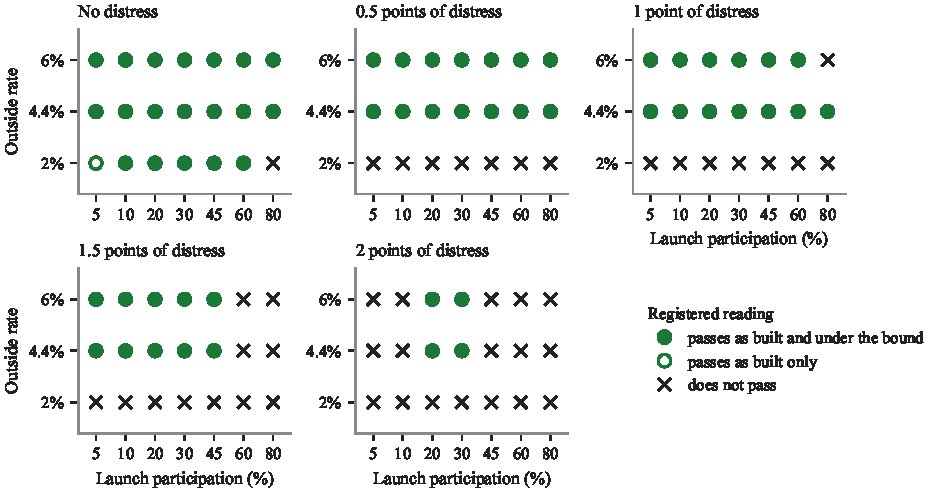
\includegraphics[width=\linewidth]{figures/fig_region.pdf}
\caption{The registered claim on the \NumSeeds{} confirmation seeds, one panel per distress level.}
\label{fig:region}
\end{figure}

\subsection{The edge at low outside rates}\label{sec:lowrates}

The registered grid has three outside rates, and the sharpest change in the claim lies between two of them: under
distress the region holds no cell at 2\% and, at half a point, every cell at 4.4\%. After the confirmation map was
read the gap was filled with a rate cut, outside rates of 2.5, 3 and 3.5\% over the same launch and distress
levels, on the frozen model and read by the same rules. It is exploratory. It was run on \CutSeedsTried{} seeds
of a block kept for runs after the confirmation, of which \CutSeeds{} completed; \CutSeedsAside{} were set
aside because one of their \CutCells{} runs stopped on a day whose settlement did not converge
(Section~\ref{sec:limits}). No clause of the registered claim reads it.

Table~\ref{tab:cut} sets the cut's rows between the registered ones. With no distress the claim passes in
\CutPassZeroTwoFive{} of seven cells at 2.5\%, \CutPassZeroThree{} at 3\% and \CutPassZeroThreeFive{} at 3.5\%, so
the edge lies between 3\% and 3.5\%. Under distress the region widens step by step with the rate: at half a point
it holds \CutPassHalfTwoFive{}, \CutPassHalfThree{} and \CutPassHalfThreeFive{} cells at the three rates, and at 1
point \CutPassOneTwoFive{}, \CutPassOneThree{} and \CutPassOneThreeFive{}. The cells that miss with no distress
miss as the cells at 2\% do, on the group clause under the cash-advance bound at the lowest launch levels and on
real cost against best-case DeFi at a launch of 80\%. Every gain is positive in \CutGainPositive{} of the cut's
\CutCells{} cells, and CPM fails fewer payments than both alternatives in \CutFewerFailures{}. Across the six
rates the gains, the bridges served and pool capital against its target all rise with the rate, with no reversal
between the grid's points. One count does not: with no distress fewer cells pass at 2.5\% (\CutPassZeroTwoFive{}) than
in the registered row at 2\% (Table~\ref{tab:cut}). The cut's rows are read on other seeds than the registered rows, and on fewer. They
locate the edge and are not a second test of the claim.

\begin{table}[htbp]\centering\footnotesize
% Written by scripts/paper_numbers.py from confirmation_quote.
\begin{tabular}{llcccccccr}
\toprule
Distress & Outside rate & 5\% & 10\% & 20\% & 30\% & 45\% & 60\% & 80\% & Cells passing \\
\midrule
0 pt & 2.0\% & $\times$ & $\bullet$ & $\bullet$ & $\bullet$ & $\bullet$ & $\bullet$ & $\times$ & 5 \\
 & 2.5\%$^{\dagger}$ & $\times$ & $\times$ & $\bullet$ & $\bullet$ & $\bullet$ & $\bullet$ & $\times$ & 4 \\
 & 3.0\%$^{\dagger}$ & $\times$ & $\bullet$ & $\bullet$ & $\bullet$ & $\bullet$ & $\bullet$ & $\times$ & 5 \\
 & 3.5\%$^{\dagger}$ & $\bullet$ & $\bullet$ & $\bullet$ & $\bullet$ & $\bullet$ & $\bullet$ & $\bullet$ & 7 \\
 & 4.4\% & $\bullet$ & $\bullet$ & $\bullet$ & $\bullet$ & $\bullet$ & $\bullet$ & $\bullet$ & 7 \\
 & 6.0\% & $\bullet$ & $\bullet$ & $\bullet$ & $\bullet$ & $\bullet$ & $\bullet$ & $\bullet$ & 7 \\
\midrule
0.5 pt & 2.0\% & $\times$ & $\times$ & $\times$ & $\times$ & $\times$ & $\times$ & $\times$ & 0 \\
 & 2.5\%$^{\dagger}$ & $\times$ & $\times$ & $\bullet$ & $\bullet$ & $\times$ & $\times$ & $\times$ & 2 \\
 & 3.0\%$^{\dagger}$ & $\times$ & $\bullet$ & $\bullet$ & $\bullet$ & $\bullet$ & $\times$ & $\times$ & 4 \\
 & 3.5\%$^{\dagger}$ & $\bullet$ & $\bullet$ & $\bullet$ & $\bullet$ & $\bullet$ & $\bullet$ & $\times$ & 6 \\
 & 4.4\% & $\bullet$ & $\bullet$ & $\bullet$ & $\bullet$ & $\bullet$ & $\bullet$ & $\bullet$ & 7 \\
 & 6.0\% & $\bullet$ & $\bullet$ & $\bullet$ & $\bullet$ & $\bullet$ & $\bullet$ & $\bullet$ & 7 \\
\midrule
1 pt & 2.0\% & $\times$ & $\times$ & $\times$ & $\times$ & $\times$ & $\times$ & $\times$ & 0 \\
 & 2.5\%$^{\dagger}$ & $\times$ & $\times$ & $\times$ & $\times$ & $\times$ & $\times$ & $\times$ & 0 \\
 & 3.0\%$^{\dagger}$ & $\times$ & $\times$ & $\bullet$ & $\bullet$ & $\times$ & $\times$ & $\times$ & 2 \\
 & 3.5\%$^{\dagger}$ & $\bullet$ & $\bullet$ & $\bullet$ & $\bullet$ & $\bullet$ & $\times$ & $\times$ & 5 \\
 & 4.4\% & $\bullet$ & $\bullet$ & $\bullet$ & $\bullet$ & $\bullet$ & $\bullet$ & $\bullet$ & 7 \\
 & 6.0\% & $\bullet$ & $\bullet$ & $\bullet$ & $\bullet$ & $\bullet$ & $\bullet$ & $\times$ & 6 \\
\midrule
1.5 pt & 2.0\% & $\times$ & $\times$ & $\times$ & $\times$ & $\times$ & $\times$ & $\times$ & 0 \\
 & 2.5\%$^{\dagger}$ & $\times$ & $\times$ & $\times$ & $\times$ & $\times$ & $\times$ & $\times$ & 0 \\
 & 3.0\%$^{\dagger}$ & $\times$ & $\times$ & $\times$ & $\times$ & $\times$ & $\times$ & $\times$ & 0 \\
 & 3.5\%$^{\dagger}$ & $\bullet$ & $\bullet$ & $\bullet$ & $\bullet$ & $\times$ & $\times$ & $\times$ & 4 \\
 & 4.4\% & $\bullet$ & $\bullet$ & $\bullet$ & $\bullet$ & $\bullet$ & $\times$ & $\times$ & 5 \\
 & 6.0\% & $\bullet$ & $\bullet$ & $\bullet$ & $\bullet$ & $\bullet$ & $\times$ & $\times$ & 5 \\
\midrule
2 pt & 2.0\% & $\times$ & $\times$ & $\times$ & $\times$ & $\times$ & $\times$ & $\times$ & 0 \\
 & 2.5\%$^{\dagger}$ & $\times$ & $\times$ & $\times$ & $\times$ & $\times$ & $\times$ & $\times$ & 0 \\
 & 3.0\%$^{\dagger}$ & $\times$ & $\times$ & $\times$ & $\times$ & $\times$ & $\times$ & $\times$ & 0 \\
 & 3.5\%$^{\dagger}$ & $\times$ & $\times$ & $\bullet$ & $\times$ & $\times$ & $\times$ & $\times$ & 1 \\
 & 4.4\% & $\times$ & $\times$ & $\bullet$ & $\bullet$ & $\times$ & $\times$ & $\times$ & 2 \\
 & 6.0\% & $\times$ & $\times$ & $\bullet$ & $\bullet$ & $\times$ & $\times$ & $\times$ & 2 \\
\bottomrule
\end{tabular}

\caption{The claim over six outside rates, by distress level and launch participation: $\bullet$ in its map's
region, $\circ$ passing outside the largest joined block, $\times$ not passing. Rates marked $\dagger$ are the
exploratory rate cut on \CutSeeds{} seeds; the others are the registered map on \NumSeeds{} seeds.}
\label{tab:cut}
\end{table}

Two things make the claim weakest at low outside rates. The first is the reserve return: there is less of it to
pass on (Table~\ref{tab:sources}), so every gain in money is smaller. The second is what is asked of the pool
(Table~\ref{tab:lending}, Figure~\ref{fig:lowrates}). The pool lends an instalment loan
only when its coupon is no dearer than the outside lender's rate on that loan. Its coupon moves one for one
with the outside rate, while the outside lender's rates on new vehicle and personal loans move by 0.75 and 0.63 of
a change in it (Section~\ref{sec:model}). So at a low outside rate the pool undercuts the outside lender on
loans it leaves to that lender at a higher one. At 2\% its instalment coupon is \LendCouponTwo{}, below the outside
lender's \LendNewCarTwo{} on new-car loans to borrowers with scores of 661 to 780 and \LendUsedCarTwo{} on used-car
loans to those with higher scores. At 4.4\% it is \LendCouponFourFour{} against \LendNewCarFourFour{} and
\LendUsedCarFourFour{}, and those loans stay with the outside lender. The cut's rates place the crossing
between 2.5\% and 3.5\%, and the edge of the region with no distress lies between 3\% and 3.5\%
(Table~\ref{tab:cut}).

These are sixty-month loans, and within a day the pool's cash goes to instalment purchases before
bridges. With them the pool lends \LendTermMore{} more in instalment loans at 2\% than at 4.4\%,
\LendTermTwo{} a person a year against \LendTermFourFour{}, and its capital target is \LendTargetMore{} higher,
\LendTargetTwo{} a person against \LendTargetFourFour{}. Capital follows the target, to \LendCapitalTwo{} of it
against \LendCapitalFourFour{}, but less cash is left for bridging: bridging refused is \LendRefusedMore{} higher,
\LendRefusedTwo{} a person a year against \LendRefusedFourFour{}, and bridges served are \LendServedTwo{} against
\LendServedFourFour{}. Every row of the table moves in one direction across the six
rates. So the weak edge at low outside rates has two sources, both stated in the model: a smaller reserve
return, and a pool whose instalment book grows when the outside lender's rates fall by less than its own coupon.
The contract studied here has no rule that keeps pool cash back for bridging when instalment lending asks for it.

\begin{table}[htbp]\centering\small
\resizebox{\linewidth}{!}{% Written by scripts/paper_numbers.py from confirmation_quote.
\begin{tabular}{lrrrrrr}
\toprule
Outside rate & 2.0\% & 2.5\%$^{\dagger}$ & 3.0\%$^{\dagger}$ & 3.5\%$^{\dagger}$ & 4.4\% & 6.0\% \\
\midrule
Pool's instalment coupon & 4.39\% & 4.90\% & 5.42\% & 5.86\% & 6.79\% & 8.38\% \\
Outside lender, new car, scores 661 to 780 & 4.55\% & 4.92\% & 5.30\% & 5.67\% & 6.35\% & 7.55\% \\
Outside lender, used car, scores 781 and above & 4.69\% & 5.06\% & 5.44\% & 5.81\% & 6.49\% & 7.69\% \\
\midrule
Pool instalment lending, \$ a person a year & \$1{,}150 & \$1{,}142 & \$1{,}103 & \$1{,}062 & \$999 & \$993 \\
Capital target, \$ a person & \$1{,}853 & \$1{,}809 & \$1{,}712 & \$1{,}534 & \$1{,}370 & \$1{,}355 \\
Pool capital over its target & 0.95 & 0.96 & 0.97 & 0.98 & 0.98 & 0.99 \\
Bridging refused, \$ a person a year & \$569 & \$525 & \$458 & \$370 & \$312 & \$294 \\
Bridges served & 0.76 & 0.78 & 0.81 & 0.85 & 0.87 & 0.88 \\
\bottomrule
\end{tabular}
}
\caption{What is asked of the pool, by outside rate with no distress. The first three rows compare the pool's
instalment coupon with the outside lender's rate on the two kinds of vehicle loan for which the comparison changes
side within these rates; the pool lends such a loan when its coupon is no dearer. The other rows are medians over
the seven launch levels. Rates marked $\dagger$ are the exploratory rate cut on \CutSeeds{} seeds; the others are
the registered map on \NumSeeds{} seeds.}
\label{tab:lending}
\end{table}

\begin{figure}[htbp]\centering
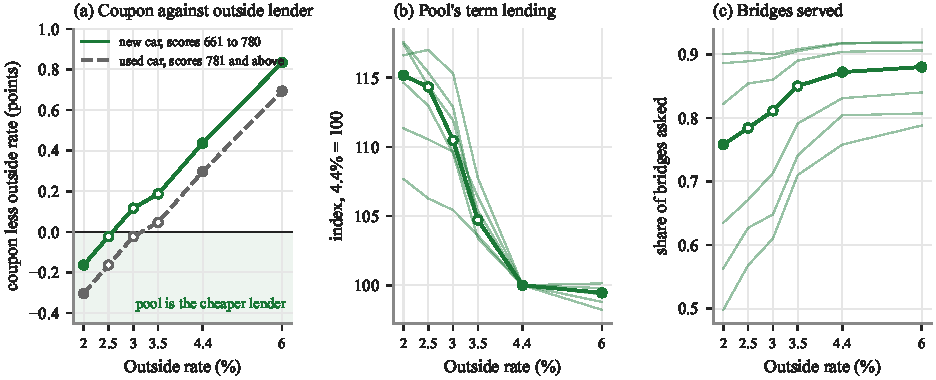
\includegraphics[width=\linewidth]{figures/fig_low_rates.pdf}
\caption{The edge at low outside rates, with no distress. (a) The pool's term coupon less the outside lender's rate
on the two kinds of vehicle loan of Table~\ref{tab:lending}; the pool lends such a loan where the difference is
not above zero. (b) The pool's term lending, each launch level set to 100 at an outside rate of 4.4\%. (c) Bridges
served. Thin lines are launch levels and the thick line their median. Hollow markers are the exploratory rate
cut.}
\label{fig:lowrates}
\end{figure}

\subsection{Stress}\label{sec:stress}

Table~\ref{tab:stress} and Figure~\ref{fig:stress} show where the result ends. Under distress the share of bridges
the pool serves in years 4 and 5 falls, and falls further the higher launch participation is. At 2 points and
an outside rate of 4.4\% a pool run, bridges served below 60\%, appears in at least one of the \NumSeeds{} seeds from \RunAdoption{}
launch participation upward; at an outside rate of 2\% runs begin at lower participation and lower distress
(Figure~\ref{fig:stress}). A run starts when a write-off takes owners' realised return below their alternative:
owners file to leave, the cash set aside for them cannot be lent, and long loans cannot be called. Bridges served
can fall below 60\% without owners leaving: with no distress they do in 1 of the \NumSeeds{} seeds at a launch of
60\% and in 6 at 80\%, where the pool is stretched (Table~\ref{tab:stress}).

Payments still fail less often under CPM on average: \FailCpmStressMean{} at 2 points of distress, against
\FailBanksStressMean{} under banks and cards and \FailDefiStressMean{} under best-case DeFi. That is
\FailCutBanksStress{} and \FailCutDefiStress{} lower, where with no distress it is \FailCutBanks{} and
\FailCutDefi{}. Across the whole grid,
by the share of payments that fail, CPM fails fewer than both alternatives in \CellsFewerFailures{} of \CellsAll{} cells. The six exceptions
all lie at an outside rate of 2\%, at launch participation of 45\% and above and distress of 1 point and above
(Figure~\ref{fig:failed}).

The gains above are earned over the whole run, which includes two years before the shock. Counting only
what is earned after it, in months 37 to 60, CPM's gain in money over banks and cards is positive in
\GainAfterBanksPositive{} of the \CellsAll{} cells, the lowest being \GainAfterBanksLow{} a person a year. Over
best-case DeFi it is positive in \GainAfterDefiPositive{}. The cells where it is negative, the lowest at
\GainAfterDefiLow{}, lie in the same corner: an outside rate of 2\%, launch participation of 45\% and above and
distress of 1.5 points and above, where owners run on the pool. There a household is still ahead over the sixty months
and is losing ground to best-case DeFi when the run ends. At 2 points the median cell earns
\GainAfterBanksMedianTwo{} a person a year over banks and cards after the shock and \GainAfterDefiMedianTwo{} over
best-case DeFi, against \GainAfterBanksMedianZero{} and \GainAfterDefiMedianZero{} over the same months with no
distress: \GainAfterBanksLowerTwo{} and \GainAfterDefiLowerTwo{} less.

The registered region narrows with distress: \RegionCellsHalf{} cells at half a point, \RegionCellsOne{} at 1
point, \RegionCellsOneHalf{} at 1.5 points and \RegionCellsTwo{} at 2 points (Table~\ref{tab:region}). At an
outside rate of 2\% no cell withstands half a point. At 4.4\% and 6\% launch levels of 20\% and 30\% withstand 2
points, launch levels of 5\%, 10\% and 45\% withstand 1.5 points, and launch levels of 60\% and 80\% withstand 1
point, or half a point at 6\% and a launch of 80\%. The claim withstands the most distress in the middle of the
launch range, and the two ends fail for different reasons. At launches of 5\% and 10\% the 2-point level fails on
clause (a): too few seeds read Persistent, though the pool still serves most of the bridges asked of it. At
launches of 45\% and above the level that fails does so on the dip in payments and on real cost, where the pool
serves about half the bridges asked of it.

\begin{figure}[htbp]\centering
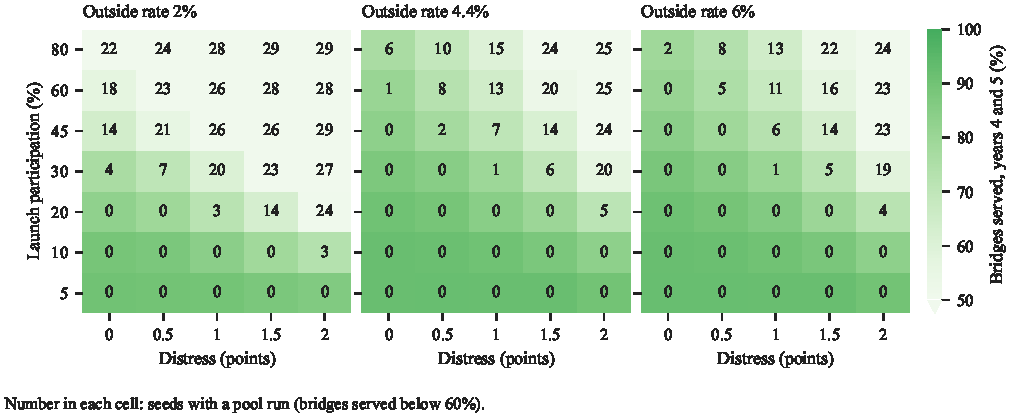
\includegraphics[width=\linewidth]{figures/fig_stress_boundary.pdf}
\caption{Bridges served under CPM in years 4 and 5, by launch participation and distress level, one panel per
outside rate. The number in each cell is the count of seeds, of \NumSeeds{}, with a pool run.}
\label{fig:stress}
\end{figure}

\begin{table}[htbp]\centering\footnotesize
\resizebox{\linewidth}{!}{% Written by scripts/paper_numbers.py from confirmation_quote.
\begin{tabular}{rrrrrrrr}
\toprule
Launch & Distress (pt) & Bridges served, years 4 and 5 & Seeds with a run (below 0.6) & Seeds below years 1 to 3 & Offers unused & Bridge write-offs (\$) & Term write-offs (\$) \\
\midrule
5\% & 0 & 0.918 & 0 of 30 & 4 of 30 & 79.4\% & \$0.4 & \$2.4 \\
5\% & 0.5 & 0.919 & 0 of 30 & 5 of 30 & 76.2\% & \$0.4 & \$3.0 \\
5\% & 1 & 0.915 & 0 of 30 & 10 of 30 & 71.7\% & \$0.4 & \$3.8 \\
5\% & 1.5 & 0.914 & 0 of 30 & 12 of 30 & 66.1\% & \$0.5 & \$4.4 \\
5\% & 2 & 0.896 & 0 of 30 & 13 of 30 & 57.4\% & \$0.9 & \$5.4 \\
10\% & 0 & 0.917 & 0 of 30 & 5 of 30 & 71.7\% & \$0.5 & \$3.3 \\
10\% & 0.5 & 0.914 & 0 of 30 & 7 of 30 & 67.2\% & \$0.6 & \$4.4 \\
10\% & 1 & 0.901 & 0 of 30 & 12 of 30 & 60.6\% & \$0.7 & \$5.5 \\
10\% & 1.5 & 0.877 & 0 of 30 & 18 of 30 & 53.1\% & \$0.8 & \$5.7 \\
10\% & 2 & 0.831 & 0 of 30 & 25 of 30 & 42.5\% & \$1.1 & \$6.4 \\
20\% & 0 & 0.904 & 0 of 30 & 13 of 30 & 61.0\% & \$0.6 & \$4.3 \\
20\% & 0.5 & 0.885 & 0 of 30 & 16 of 30 & 53.9\% & \$0.8 & \$5.3 \\
20\% & 1 & 0.843 & 0 of 30 & 23 of 30 & 45.2\% & \$0.9 & \$6.4 \\
20\% & 1.5 & 0.796 & 0 of 30 & 28 of 30 & 35.0\% & \$1.1 & \$7.0 \\
20\% & 2 & 0.708 & 5 of 30 & 29 of 30 & 23.2\% & \$1.4 & \$8.9 \\
30\% & 0 & 0.872 & 0 of 30 & 19 of 30 & 52.8\% & \$0.7 & \$5.3 \\
30\% & 0.5 & 0.845 & 0 of 30 & 20 of 30 & 44.5\% & \$1.0 & \$5.9 \\
30\% & 1 & 0.794 & 1 of 30 & 26 of 30 & 34.8\% & \$1.2 & \$7.7 \\
30\% & 1.5 & 0.698 & 6 of 30 & 30 of 30 & 23.2\% & \$1.4 & \$7.8 \\
30\% & 2 & 0.564 & 20 of 30 & 30 of 30 & 12.9\% & \$1.3 & \$9.6 \\
45\% & 0 & 0.831 & 0 of 30 & 24 of 30 & 45.7\% & \$1.0 & \$5.3 \\
45\% & 0.5 & 0.774 & 2 of 30 & 28 of 30 & 35.9\% & \$1.4 & \$6.4 \\
45\% & 1 & 0.702 & 7 of 30 & 28 of 30 & 24.0\% & \$1.5 & \$7.2 \\
45\% & 1.5 & 0.613 & 14 of 30 & 29 of 30 & 13.1\% & \$1.6 & \$8.0 \\
45\% & 2 & 0.453 & 24 of 30 & 29 of 30 & 4.5\% & \$1.7 & \$9.3 \\
60\% & 0 & 0.804 & 1 of 30 & 21 of 30 & 42.9\% & \$1.2 & \$6.2 \\
60\% & 0.5 & 0.725 & 8 of 30 & 23 of 30 & 31.9\% & \$1.3 & \$7.0 \\
60\% & 1 & 0.643 & 13 of 30 & 27 of 30 & 20.7\% & \$1.5 & \$7.8 \\
60\% & 1.5 & 0.523 & 20 of 30 & 28 of 30 & 11.7\% & \$1.8 & \$8.8 \\
60\% & 2 & 0.384 & 25 of 30 & 29 of 30 & 5.1\% & \$1.6 & \$11 \\
80\% & 0 & 0.758 & 6 of 30 & 20 of 30 & 37.5\% & \$1.3 & \$5.0 \\
80\% & 0.5 & 0.687 & 10 of 30 & 22 of 30 & 27.4\% & \$1.5 & \$6.6 \\
80\% & 1 & 0.597 & 15 of 30 & 24 of 30 & 16.6\% & \$1.5 & \$7.3 \\
80\% & 1.5 & 0.461 & 24 of 30 & 27 of 30 & 9.6\% & \$1.8 & \$8.8 \\
80\% & 2 & 0.329 & 25 of 30 & 29 of 30 & 4.4\% & \$1.8 & \$10 \\
\bottomrule
\end{tabular}
}
\caption{CPM under distress at an outside rate of 4.4\%: bridges served in years 4 and 5, the seeds with a pool run,
the seeds whose bridges served fall below their own level in years 1 to 3, the share of offers to the pool left
unused, and write-offs in dollars a person a year.}
\label{tab:stress}
\end{table}

\subsection{When savers judge the pool by its record}\label{sec:record}

The confirmation map was run again on the same seeds with one rule changed. Under the quote rule, the
decided one, a saver who reviews entry offers its money when the pool's published quote is at least the saver's
alternative. Under the record rule it does so when the pool's realised return over the last twelve months is.
The record rule is the pessimistic reading of the condition in Proposition~\ref{prop:capital}.
Table~\ref{tab:readings} sets the two rules side by side.

CPM stays ahead of both alternatives under either rule. Every gain over banks and cards and over best-case DeFi is
positive in \ReadSecondGainPositive{} of the \CellsAll{} cells of the grid. The median gain is
\ReadSecondGainBanks{} a person a year over banks and cards and \ReadSecondGainDefi{} over best-case DeFi,
\ReadSecondGainBanksLower{} and \ReadSecondGainDefiLower{} below the gains under the quote rule. CPM
fails \ReadSecondFailCpm{} of payments against \ReadSecondFailBanks{} under banks and cards. The real-cost clause
and the group clause pass in all \CellsNoDistress{} cells with no distress, as built and under the cash-advance
bound, and no falsifier fires.

The rule decides whether the pool sustains itself. Over years 4 and 5 pool capital stands at
\ReadSecondCapital{} of its target, against \ReadFirstCapital{} under the quote rule, and the pool serves
\ReadSecondServedCpm{} of the bridges asked of it, against \ReadFirstServedCpm{}. The pool is Persistent in \ReadSecondPersistentLow{} to
\ReadSecondPersistentHigh{} of the \NumSeeds{} seeds, depending on the cell, where clause (a) needs
\WilsonConfirm{}. That clause fails in all but \ReadSecondRegion{} cells, so under this reading the registered
claim holds in \ReadSecondRegion{} of the \CellsNoDistress{} cells with no distress and in none under distress.
The condition of Proposition~\ref{prop:capital} is the knife-edge of the design, and these numbers are its size.

Neither level of capital is a resting point. Table~\ref{tab:path} follows the pool year by year and Figure~\ref{fig:path} month by month. Its capital target rises
throughout the run under both rules, as the network grows and the term book fills: the longest loans run
sixty months, so the book is still filling when the run ends. Under the quote rule capital follows the
target to within one per cent for four years and stands at \PathFirstRatioFive{} of it in the fifth. Under the
record rule capital falls behind from the first year. It is \PathSecondRatioFour{} of the target in year 4
and \PathSecondRatioFive{} in year 5, and bridges served fall from \PathSecondServedFour{} to
\PathSecondServedFive{}. Capital still grows in dollars, from \PathSecondCapitalFour{} to \PathSecondCapitalFive{}
a person, but more slowly than what is asked of it. So sixty months do not show where the pool comes to
rest under this reading, only that it has not come to rest and is still losing ground when the run ends.

The record rule is also where demurrage does most. Without the charge the pool serves \ReadSecondServedPool{} of
bridges at a price of \ReadSecondPricePool{} and fails \ReadSecondFailPool{} of payments, close to the bank
arrangement. With the charge it serves \ReadSecondServedCpm{} at \ReadSecondPriceCpm{}. CPM's gain over the pool
without the charge is \ReadSecondGainOverPool{} a person a year under this reading, against
\ReadFirstGainOverPool{} under the quote rule. The two maps share their seeds and the bank arrangement is
the same in both, so they are one body of evidence read under two assumptions, not two confirmations.

\begin{table}[htbp]\centering\small
% Written by scripts/paper_numbers.py from confirmation_quote.
\begin{tabular}{lrr}
\toprule
 & Quote rule & Record rule \\
\midrule
Cells in the registered region, no distress & 19 & 2 \\
Seeds in which the pool persists & 26 to 30 & 6 to 23 \\
Pool capital over its target & 0.97 & 0.77 \\
\midrule
Bridges served, CPM & 0.84 & 0.52 \\
Bridges served, pool without the charge & 0.77 & 0.17 \\
Bridge price, CPM & 2.1\% & 2.4\% \\
Bridge price, pool without the charge & 6.7\% & 11.4\% \\
Payments that fail, banks and cards & 3.65\% & 3.65\% \\
Payments that fail, pool without the charge & 2.59\% & 3.35\% \\
Payments that fail, CPM & 2.51\% & 2.86\% \\
Gain over banks and cards & \$262 & \$217 \\
Gain over best-case DeFi & \$140 & \$90 \\
Gain over the pool without the charge & \$15 & \$61 \\
\midrule
Cells of the grid with every gain positive & 105 & 105 \\
Cells of the grid with fewer failed payments than both & 99 & 98 \\
\bottomrule
\end{tabular}

\caption{The confirmation map under the two entry rules, on the same \NumSeeds{} seeds: medians over
the \CellsNoDistress{} cells with no distress, and counts of cells. The second row is the range over those cells of
the number of seeds, of \NumSeeds{}, where the pool reads Persistent.}
\label{tab:readings}
\end{table}

\begin{table}[htbp]\centering\small
\resizebox{\linewidth}{!}{% Written by scripts/paper_numbers.py from confirmation_quote.
\begin{tabular}{lrrrrrrrr}
\toprule
 & \multicolumn{4}{c}{Quote rule} & \multicolumn{4}{c}{Record rule} \\
Year after launch & Capital over target & Capital, \$ & Target, \$ & Bridges served & Capital over target & Capital, \$ & Target, \$ & Bridges served \\
\midrule
1 & 1.01 & \$293 & \$292 & 0.87 & 0.97 & \$287 & \$298 & 0.81 \\
2 & 1.00 & \$614 & \$611 & 0.90 & 0.91 & \$563 & \$630 & 0.72 \\
3 & 1.00 & \$899 & \$895 & 0.90 & 0.91 & \$792 & \$884 & 0.70 \\
4 & 1.00 & \$1{,}284 & \$1{,}286 & 0.88 & 0.85 & \$1{,}040 & \$1{,}241 & 0.59 \\
5 & 0.96 & \$1{,}653 & \$1{,}728 & 0.80 & 0.75 & \$1{,}152 & \$1{,}564 & 0.43 \\
\bottomrule
\end{tabular}
}
\caption{The pool year by year after launch under the two entry rules, with no distress: for each
year the median over the \CellsNoDistress{} cells of the seed mean of the year's months. Capital and its target
are in dollars a person.}
\label{tab:path}
\end{table}

\begin{figure}[htbp]\centering
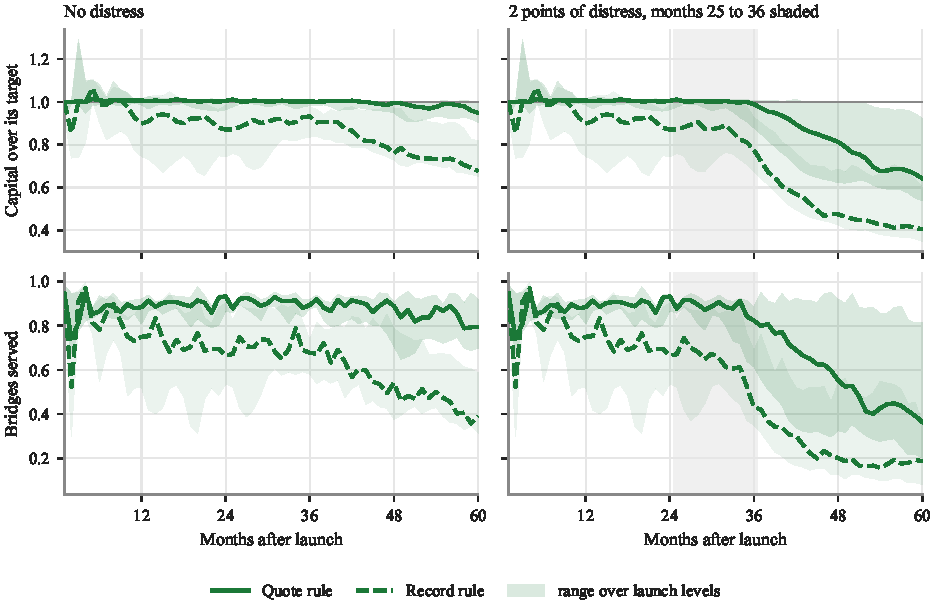
\includegraphics[width=\linewidth]{figures/fig_path.pdf}
\caption{Pool capital over its target (top) and bridges served (bottom), month by month after launch at an outside
rate of 4.4\%, under the quote rule and the record rule: the median over the seven launch levels of each cell's
seed mean, and their range. Left, no distress; right, 2 points of distress.}
\label{fig:path}
\end{figure}
